% ============================================================
%  Presentación Beamer — Metaheurísticas para el LRP
%  Semana 10: Fuerza Bruta + ALNS + MA|PM + Validación
% ============================================================
\documentclass[aspectratio=169,10pt]{beamer}

\usepackage[T1]{fontenc}
\usepackage[utf8]{inputenc}

\usetheme{Madrid}
\usecolortheme{whale}
\usefonttheme[onlymath]{serif}

\usepackage{amsmath,amssymb}
\usepackage{booktabs}
\usepackage{xcolor}
\usepackage{tikz}
\usetikzlibrary{positioning,shapes.geometric,arrows.meta,calc,fit}
\usepackage{pgfplots}
\pgfplotsset{compat=1.18}
\usepackage{algorithm}
\usepackage{algpseudocode}
\usepackage{colortbl}
\renewcommand{\algorithmicrequire}{\textbf{Entrada:}}
\renewcommand{\algorithmicensure}{\textbf{Salida:}}

\definecolor{myblue}{RGB}{0,70,127}
\definecolor{mygreen}{RGB}{0,130,0}
\definecolor{myorange}{RGB}{200,100,0}

\newcommand{\tc}[1]{\texttt{\small #1}}
% (Beamer ya define \tt, usamos \tc para monospace)

\title[Metaheurísticas para el LRP]{%
  Diseño e Implementación de Metaheurísticas\\
  para el \textit{Location Routing Problem}}
\subtitle{Fuerza Bruta · ALNS · MA$|$PM --- Implementación en C++17}
\author[Lizárraga \& Loayza]{%
  Sebastián Andre Lizárraga Calderón \and
  Johannes Albert Loayza Huamán}
\date{\today}

\setbeamertemplate{navigation symbols}{}
\setbeamertemplate{footline}[frame number]

% \tt ya definido en Beamer; usar \tc

% ============================================================
\begin{document}

\begin{frame}
  \titlepage
\end{frame}

\begin{frame}{Agenda}
  \tableofcontents
\end{frame}

% ============================================================
\section{Arquitectura del Software}

\begin{frame}{Estructura del Proyecto}
  \begin{columns}[T,onlytextwidth]
    \begin{column}{0.42\textwidth}
      \textbf{Tres bibliotecas CMake:}
      \vspace{0.3em}
      \begin{block}{\tc{lrp\_core} --- Dominio}
        \footnotesize
        \begin{itemize}
          \item \tc{parser}: lee archivos \texttt{.dat} (Prodhon)
          \item \tc{distancia}: matriz euclidiana $d_{ij}$
          \item \tc{estado}: \tc{EstadoLRP} + función objetivo
          \item \tc{solucion\_inicial}: greedy All-Open
        \end{itemize}
      \end{block}
      \begin{block}{\tc{alns\_lib}}
        \footnotesize \tc{operadores} $\to$ \tc{alns} $\to$ \tc{solver}
      \end{block}
      \begin{block}{\tc{mapm\_lib}}
        \footnotesize \tc{cromosoma} $\to$ \tc{split} $\to$
        \tc{poblacion} $\to$ \tc{local\_search}
      \end{block}
    \end{column}
    \begin{column}{0.56\textwidth}
      \textbf{Interfaz común \tc{IAlgoritmo}:}
      \vspace{0.3em}
      \begin{center}
      \resizebox{0.88\textwidth}{!}{%
      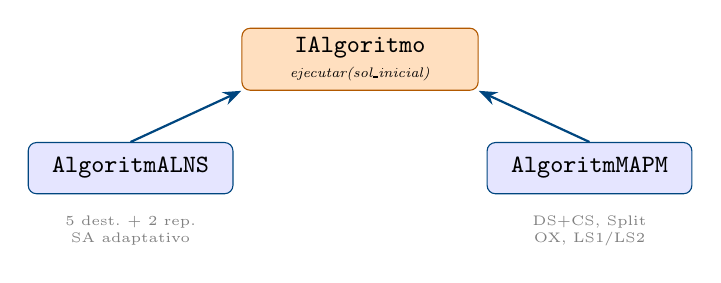
\begin{tikzpicture}[
        box/.style={rectangle, rounded corners=3pt, draw=myblue, fill=blue!10,
                    minimum width=2.6cm, minimum height=0.65cm,
                    font=\small, align=center},
        arr/.style={-{Stealth}, thick, myblue}
      ]
        \node[box, fill=orange!25, draw=orange!70!black, minimum width=3.0cm] (iface)
              {\tc{IAlgoritmo}\\[-2pt]\tiny\textit{ejecutar(sol\_inicial)}};
        \node[box, below left=0.65cm and 0.1cm of iface] (alns)
              {\tc{AlgoritmALNS}};
        \node[box, below right=0.65cm and 0.1cm of iface] (mapm)
              {\tc{AlgoritmMAPM}};
        \draw[arr] (alns.north) -- (iface.south west);
        \draw[arr] (mapm.north) -- (iface.south east);
        \node[below=0.15cm of alns, font=\tiny\color{gray}, align=center]
              {5 dest.\ + 2 rep.\\SA adaptativo};
        \node[below=0.15cm of mapm, font=\tiny\color{gray}, align=center]
              {DS+CS, Split\\OX, LS1/LS2};
      \end{tikzpicture}}
      \end{center}
      \vspace{0.15em}
      \textbf{Función objetivo:}
      \[
        Z = \underbrace{\textstyle\sum_{i \in D_{open}} O_i}_{apertura}
          + \underbrace{\textstyle\sum_{r} (F + \text{dist}(r))}_{rutas}
          + 10^6 \cdot |\textit{no-asig}|
      \]
    \end{column}
  \end{columns}
\end{frame}

\begin{frame}{Tipos Principales}
  \begin{columns}[T,onlytextwidth]
    \begin{column}{0.48\textwidth}
      \begin{block}{\tc{EstadoLRP} --- Solución}
        \footnotesize
        \begin{itemize}
          \item \tc{rutas}: \texttt{map<depot\_id, vector<Ruta>}
          \item \tc{depositos\_abiertos}: conjunto de IDs activos
          \item \tc{no\_asignados}: clientes sin ruta
          \item \tc{*matriz}, \tc{*datos}: punteros \textbf{no-owning}
          \item \tc{.copy()}: copia profunda de rutas
        \end{itemize}
        \vspace{0.1em}
        \textbf{Convención:} clientes $1\ldots n_c$;
        depósitos $n_c{+}1\ldots n_c{+}n_d$. Matriz 0-indexed.
      \end{block}
      \begin{block}{\tc{struct Ruta} --- Circuito de un vehículo}
        \footnotesize
        \begin{itemize}
          \item \tc{id\_deposito}: depósito que origina la ruta
          \item \tc{clientes}: \texttt{vector<int>} de IDs 1-indexed
          \item \tc{costo}: distancia total $+F$ del circuito
          \item \tc{demanda\_acumulada}: suma de $d_j$ en la ruta
        \end{itemize}
      \end{block}
    \end{column}
    \begin{column}{0.50\textwidth}
      \begin{block}{\tc{CromosomaLRP} (MA$|$PM)}
        \footnotesize
        \begin{itemize}
          \item \tc{DS[0..m-1]}: estado de depósitos (0-indexed).
                Valor $>0$ = abierto; 0 = cerrado.
          \item \tc{CS[0..n-1]}: permutación de clientes (\textit{giant tour})
          \item \tc{fitness}: costo decodificado por Split
        \end{itemize}
      \end{block}
      \begin{block}{\tc{ResultadoAlgoritmo}}
        \footnotesize
        \begin{itemize}
          \item \tc{mejor\_estado}: \tc{EstadoLRP} óptimo hallado
          \item \tc{costo\_inicial} / \tc{costo\_final}
          \item \tc{iteraciones}, \tc{historial\_mejoras}
        \end{itemize}
      \end{block}
    \end{column}
  \end{columns}
\end{frame}

% ============================================================
\section{Algoritmo de Fuerza Bruta}

\begin{frame}{Fuerza Bruta --- Estrategia Exacta para LRP}
  \begin{columns}[T,onlytextwidth]
    \begin{column}{0.48\textwidth}
      \textbf{El LRP tiene dos decisiones anidadas:}
      \vspace{0.3em}
      \begin{enumerate}\small
        \item \textbf{¿Qué depósitos abrir?}
              → enumerar los $2^m{-}1$ subconjuntos no vacíos
        \item \textbf{¿Cómo partir los clientes en rutas?}
              → dos DPs anidados:
      \end{enumerate}
      \vspace{0.4em}
      \begin{description}[\textbf{Set-Cover DP}]\footnotesize
        \item[\textbf{Held-Karp DP}] Dada una ruta con $k$ clientes,
              halla el orden óptimo en $\mathcal{O}(2^k \cdot k^2)$
        \item[\textbf{Set-Cover DP}] Dada la tabla de costos de rutas,
              halla la partición óptima de clientes en $\mathcal{O}(3^k)$
      \end{description}
      \vspace{0.4em}
      \begin{alertblock}{Complejidad total}
        \footnotesize $\mathcal{O}(2^m \cdot 3^n)$ --- exacto, pero exponencial.\\
        Útil como \textbf{validador} para $n \le 20$.
      \end{alertblock}
    \end{column}
    \begin{column}{0.50\textwidth}
      \vspace{0.3em}
      \begin{center}
      \resizebox{0.9\textwidth}{!}{%
      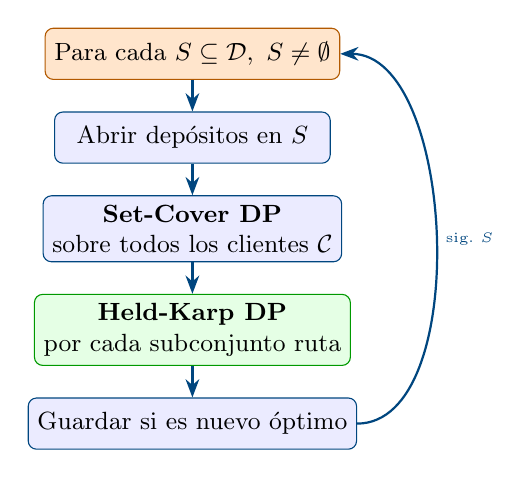
\begin{tikzpicture}[
        box/.style={rectangle, rounded corners=3pt, draw=myblue, fill=blue!8,
                    minimum width=3.5cm, minimum height=0.65cm,
                    font=\small, align=center},
        arr/.style={-{Stealth}, thick, myblue}
      ]
        \node[box, fill=orange!20, draw=orange!70!black] (s1)
              {Para cada $S \subseteq \mathcal{D},\ S\neq\emptyset$};
        \node[box, below=0.4cm of s1] (s2) {Abrir depósitos en $S$};
        \node[box, below=0.4cm of s2] (s3)
              {\textbf{Set-Cover DP}\\sobre todos los clientes $\mathcal{C}$};
        \node[box, below=0.4cm of s3, fill=green!10, draw=green!60!black] (s4)
              {\textbf{Held-Karp DP}\\por cada subconjunto ruta};
        \node[box, below=0.4cm of s4] (s5)
              {Guardar si es nuevo óptimo};
        \draw[arr] (s1)--(s2); \draw[arr] (s2)--(s3);
        \draw[arr] (s3)--(s4); \draw[arr] (s4)--(s5);
        \draw[arr] (s5.east) to[out=0,in=0,looseness=0.8]
              node[right,font=\tiny]{sig.\ $S$} (s1.east);
      \end{tikzpicture}}
      \end{center}
    \end{column}
  \end{columns}
\end{frame}

\begin{frame}{Held-Karp DP --- Orden Óptimo de una Ruta}
  \begin{columns}[T,onlytextwidth]
    \begin{column}{0.54\textwidth}
      \begin{algorithm}[H]
        \caption{\small Held-Karp: costo mínimo de ruta}
        \begin{algorithmic}[1]\tiny
          \Require clientes $R{=}\{r_0\ldots r_{k-1}\}$, depósito $D$, dist.\ $d$, costo fijo $F$
          \Ensure  costo mínimo de recorrer $R$ y volver a $D$
          \State \texttt{hk[mask][last]} $\gets +\infty$ para todo (mask, last)
          \For{$i \gets 0$ \textbf{to} $k{-}1$}
            \State \texttt{hk[$1{\ll}i$][$i$]} $\gets d[D][r_i]$
            \Comment{ruta de 1 cliente}
          \EndFor
          \For{mask $\gets 1$ \textbf{to} $2^k{-}1$}
            \For{last : bit activo en mask, \texttt{hk[mask][last]}${\ne}+\infty$}
              \For{$j \gets 0$ \textbf{to} $k{-}1$, $j \notin$ mask}
                \State $m' \gets$ mask $|$ ($1{\ll}j$)
                \State \texttt{hk[$m'$][$j$]} $\gets \min\bigl($\texttt{hk[$m'$][$j$]},\
                        \texttt{hk[mask][last]} $+ d[r_{last}][r_j]\bigr)$
              \EndFor
            \EndFor
          \EndFor
          \State full $\gets 2^k{-}1$
          \State \Return $F + \displaystyle\min_{\text{last}}\bigl($\texttt{hk[full][last]} $+ d[r_{last}][D]\bigr)$
        \end{algorithmic}
      \end{algorithm}
    \end{column}
    \begin{column}{0.44\textwidth}
      \textbf{Variables:}
      \vspace{0.2em}
      \begin{description}[\texttt{hk[mask][last]}]\footnotesize
        \item[\texttt{mask}] Máscara de bits: bit $i$ activo $\Leftrightarrow$ $r_i$ ya visitado en el recorrido parcial
        \item[\texttt{last}] Índice (en $R$) del último cliente visitado
        \item[\texttt{hk[mask][last]}] Mínimo costo de recorrer exactamente los clientes en \texttt{mask}, terminando en $r_{\text{last}}$ (sin retorno al depósito)
        \item[$F$] Costo fijo del vehículo, sumado al cerrar
      \end{description}
      \vspace{0.4em}
      \begin{exampleblock}{Ejemplo: ruta $\{C_2, C_3\}$ desde $D_2$}
        \footnotesize
        \texttt{hk[01][0]} $= d[D_2][C_2]$ \\
        \texttt{hk[10][1]} $= d[D_2][C_3]$ \\
        \texttt{hk[11][1]} $= d[D_2][C_2]+d[C_2][C_3]$ \\
        Retorno: \texttt{hk[11][1]}$+d[C_3][D_2]+F$
      \end{exampleblock}
    \end{column}
  \end{columns}
\end{frame}

\begin{frame}{Set-Cover DP --- Partición Óptima en Rutas}
  \begin{columns}[T,onlytextwidth]
    \begin{column}{0.54\textwidth}
      \begin{algorithm}[H]
        \caption{\small Set-Cover: mínimo costo para cubrir todos los clientes}
        \begin{algorithmic}[1]\tiny
          \Require clientes $C{=}\{c_0\ldots c_{n-1}\}$, depósito $D$, capacidad $Q$, dist.\ $d$
          \Ensure  costo total mínimo de cubrir $C$ con rutas desde $D$
          \ForAll{subconj. $T \subseteq C$ con demanda$(T) \le Q$}
            \State \texttt{rc[$T$]} $\gets$ Held-Karp($T$, $D$, $d$)
            \Comment{precalcular todas las rutas}
          \EndFor
          \State $dp[0] \gets 0$;\ $dp[$mask$] \gets +\infty$ para mask $> 0$
          \For{mask $\gets 1$ \textbf{to} $2^n{-}1$}
            \State sub $\gets$ mask
            \While{sub $> 0$}
              \If{demanda(sub) $\le Q$}
                \State rest $\gets$ mask $\oplus$ sub
                \State $dp[$mask$] \gets \min\bigl(dp[$mask$],\ dp[$rest$]+$\texttt{rc[sub]}$\bigr)$
              \EndIf
              \State sub $\gets$ (sub${-}1$) $\&$ mask
              \Comment{siguiente sub-máscara}
            \EndWhile
          \EndFor
          \State \Return $O(D) + dp[2^n{-}1]$
        \end{algorithmic}
      \end{algorithm}
    \end{column}
    \begin{column}{0.44\textwidth}
      \textbf{Variables:}
      \vspace{0.2em}
      \begin{description}[\texttt{dp[mask]}]\footnotesize
        \item[\texttt{rc[T]}] Costo de Held-Karp del subconjunto $T$ de clientes (incluye $F$)
        \item[\texttt{mask}] Subconjunto de clientes a cubrir (representado como máscara de bits)
        \item[\texttt{sub}] Posible ``última ruta'': cualquier sub-máscara de \texttt{mask}
        \item[\texttt{rest}] mask\;$\oplus$\;sub: clientes ya cubiertos antes de agregar \texttt{sub}
        \item[\texttt{dp[mask]}] Costo mínimo de cubrir exactamente los clientes de \texttt{mask}
      \end{description}
      \vspace{0.3em}
      \begin{alertblock}{¿Por qué $3^n$?}\footnotesize
        Cada cliente puede estar en \texttt{rest}, en \texttt{sub} o fuera de \texttt{mask}. Son 3 opciones por cliente $\Rightarrow \mathcal{O}(3^n)$.
      \end{alertblock}
    \end{column}
  \end{columns}
\end{frame}

% ============================================================
\section{ALNS: Adaptive Large Neighborhood Search}

\begin{frame}{ALNS --- Loop Principal y Simulated Annealing}
  \begin{columns}[T,onlytextwidth]
    \begin{column}{0.50\textwidth}
      \begin{algorithm}[H]
        \caption{\small Loop ALNS}
        \begin{algorithmic}[1]\tiny
          \Require solución inicial $s_0$, parámetros SA $(T_0, \alpha)$
          \Ensure  mejor solución encontrada $s^*$
          \State $s \gets s_0$;\ $s^* \gets s_0$;\ $\mathcal{T} \gets T_0$
          \While{iter $<$ max\_iter}
            \State \textit{d} $\gets$ seleccionar destructor (ruleta por pesos $w_d$)
            \State \textit{r} $\gets$ seleccionar reparador (ruleta por pesos $w_r$)
            \State $s' \gets r(d(s))$
            \If{$f(s') < f(s^*)$}
              \State $s^* \gets s'$;\ $s \gets s'$;\ score $\gets \sigma_1$
            \ElsIf{$f(s') < f(s)$}
              \State $s \gets s'$;\ score $\gets \sigma_2$
            \ElsIf{$U(0,1) < \exp\!\bigl(-\frac{f(s')-f(s)}{\mathcal{T}}\bigr)$}
              \State $s \gets s'$;\ score $\gets \sigma_3$
            \Else
              \State score $\gets \sigma_4$
            \EndIf
            \State $\pi_d \mathrel{+}=$ score;\ $\pi_r \mathrel{+}=$ score
            \State $\mathcal{T} \gets \alpha \cdot \mathcal{T}$
            \If{iter $\bmod\, T_{seg} = 0$}
              \State $w_i \gets w_i(1-\rho)+\rho\,(\pi_i/\theta_i)$ para cada op.\ $i$
              \State resetear $\pi_i, \theta_i$
            \EndIf
          \EndWhile
          \State \Return $s^*$
        \end{algorithmic}
      \end{algorithm}
    \end{column}
    \begin{column}{0.48\textwidth}
      \textbf{Parámetros de referencia:}
      \vspace{0.2em}
      \begin{center}\footnotesize
      \begin{tabular}{ll}
        \toprule
        Parámetro & Valor \\
        \midrule
        $T_0$ (temperatura inicial)    & 50\,000 \\
        $T_{end}$ (temperatura final)  & 1 \\
        $\alpha$ (enfriamiento)        & 0.998 \\
        $\rho$ (olvido de pesos)       & 0.1 \\
        $T_{seg}$ (segmento adaptivo)  & 100 iter \\
        $\sigma_1$ (nuevo mejor)       & 33 \\
        $\sigma_2$ (mejora global)     & 9 \\
        $\sigma_3$ (aceptado por SA)   & 13 \\
        $\sigma_4$ (rechazado)         & 1 \\
        Iteraciones totales            & 5\,000 \\
        \bottomrule
      \end{tabular}
      \end{center}
      \vspace{0.2em}
      \small La \textbf{ruleta adaptativa} ajusta cada $T_{seg}$
      iteraciones los pesos de operadores según su rendimiento acumulado.
    \end{column}
  \end{columns}
\end{frame}

\begin{frame}{ALNS --- Operadores de Destrucción}
  \begin{columns}[T,onlytextwidth]
    \begin{column}{0.50\textwidth}
      \begin{algorithm}[H]
        \caption{\small \texttt{random\_removal}($s$, $q$)}
        \begin{algorithmic}[1]\tiny
          \Require solución $s$, cantidad a remover $q$
          \Ensure  $s$ con $q$ clientes en \texttt{no\_asignados}
          \For{$i \gets 1$ \textbf{to} $q$}
            \State $c \gets$ cliente aleatorio de alguna ruta de $s$
            \State eliminar $c$ de su ruta
            \State agregar $c$ a \texttt{no\_asignados}
            \If{ruta queda vacía}
              \State eliminar la ruta (depósito sigue abierto)
            \EndIf
          \EndFor
          \State \Return $s$
        \end{algorithmic}
      \end{algorithm}
      \vspace{0.2em}
      \begin{algorithm}[H]
        \caption{\small \texttt{worst\_removal}($s$, $q$)}
        \begin{algorithmic}[1]\tiny
          \For{$i \gets 1$ \textbf{to} $q$}
            \State $c^* \gets \arg\max_{c}$ (costo marginal de $c$ en su ruta)
            \State eliminar $c^*$; agregar a \texttt{no\_asignados}
          \EndFor
          \State \Return $s$
        \end{algorithmic}
      \end{algorithm}
    \end{column}
    \begin{column}{0.48\textwidth}
      \textbf{Catálogo completo de destructores:}
      \vspace{0.3em}
      \begin{description}[\texttt{depot\_closing}]\footnotesize
        \item[\texttt{random\_removal}] Extrae $q$ clientes al azar
        \item[\texttt{worst\_removal}] Extrae los $q$ clientes de mayor costo marginal
        \item[\texttt{shaw\_removal}] Agrupa clientes geográficamente afines (vecindad Shaw)
        \item[\texttt{route\_removal}] Elimina una ruta completa al azar
        \item[\texttt{depot\_closing}] \textbf{Decisión de localización}: cierra un depósito y reasigna todos sus clientes
      \end{description}
      \vspace{0.3em}
      \begin{alertblock}{Limitación en LRP}\footnotesize
        \texttt{depot\_closing} puede cerrar un depósito, pero los reparadores \textbf{no pueden reabrirlo}. Si SA acepta el cierre temprano, el algoritmo queda atrapado en soluciones sub-óptimas.
      \end{alertblock}
    \end{column}
  \end{columns}
\end{frame}

\begin{frame}{ALNS --- Operadores de Reparación}
  \begin{columns}[T,onlytextwidth]
    \begin{column}{0.50\textwidth}
      \begin{algorithm}[H]
        \caption{\small \texttt{greedy\_repair}($s$)}
        \begin{algorithmic}[1]\tiny
          \Require $s$ con clientes en \texttt{no\_asignados}
          \Ensure  $s$ con todos los clientes insertados
          \While{\texttt{no\_asignados} $\ne \emptyset$}
            \State $\Delta^* \gets +\infty$;\ $c^*, \text{pos}^* \gets$ nulo
            \ForAll{$c \in$ \texttt{no\_asignados}}
              \ForAll{depósito $d \in$ \texttt{depositos\_abiertos}}
                \ForAll{ruta $r$ de depósito $d$}
                  \ForAll{posición $p$ en $r$}
                    \State $\Delta \gets$ costo adicional de insertar $c$ en $p$
                    \If{$\Delta < \Delta^*$ y demanda$(r)+1 \le Q$}
                      \State $\Delta^* \gets \Delta$;\ $c^*, \text{pos}^* \gets c, p$
                    \EndIf
                  \EndFor
                \EndFor
              \EndFor
            \EndFor
            \State Insertar $c^*$ en pos$^*$;\ quitar de \texttt{no\_asignados}
          \EndWhile
        \end{algorithmic}
      \end{algorithm}
    \end{column}
    \begin{column}{0.48\textwidth}
      \begin{algorithm}[H]
        \caption{\small \texttt{regret2\_repair}($s$)}
        \begin{algorithmic}[1]\tiny
          \While{\texttt{no\_asignados} $\ne \emptyset$}
            \ForAll{$c \in$ \texttt{no\_asignados}}
              \State $\Delta_1(c) \gets$ mejor inserción de $c$
              \State $\Delta_2(c) \gets$ segunda mejor inserción de $c$
              \State arrepentimiento$(c) \gets \Delta_2(c) - \Delta_1(c)$
            \EndFor
            \State $c^* \gets \arg\max_c$ arrepentimiento$(c)$
            \State Insertar $c^*$ en su mejor posición
          \EndWhile
        \end{algorithmic}
      \end{algorithm}
      \vspace{0.3em}
      \begin{block}{Diferencia clave}\footnotesize
        \textbf{Greedy}: inserta siempre el cliente con menor $\Delta$ inmediato (miope).\\[0.3em]
        \textbf{Regret-2}: prioriza el cliente que \textit{más perdería} si espera (con visión de futuro).
      \end{block}
    \end{column}
  \end{columns}
\end{frame}

% ============================================================
\section{MA$|$PM: Algoritmo Memético}

\begin{frame}{MA$|$PM --- Cromosoma Giant-Tour (DS + CS)}
  \begin{columns}[T,onlytextwidth]
    \begin{column}{0.50\textwidth}
      \textbf{Representación de un individuo:}
      \vspace{0.3em}
      \begin{description}[\textbf{CS (Client Sequence)}]\small
        \item[\textbf{DS (Depot State)}] Vector de $m$ enteros. DS$[i]>0$ $\Rightarrow$ depósito $i$ abierto; DS$[i]=0$ $\Rightarrow$ cerrado.
        \item[\textbf{CS (Client Sequence)}] Permutación de los $n$ clientes: el \textit{tour gigante} sin indicar depósitos ni rutas.
      \end{description}
      \vspace{0.4em}
      \begin{block}{¿Para qué sirve el Split?}\small
        DS solo dice \textbf{qué depósitos están abiertos}.\\
        CS dice \textbf{en qué orden están los clientes}.\\
        El \textbf{Split} es quien determina la partición óptima en rutas y la asignación de clientes a depósitos.
      \end{block}
    \end{column}
    \begin{column}{0.48\textwidth}
      \textbf{Ejemplo con $n=5$, $m=3$:}
      \vspace{0.3em}
      \begin{center}\footnotesize
      \begin{tabular}{ccc}
        \toprule
        DS[0] & DS[1] & DS[2] \\
        \midrule
        \textbf{1} & \textbf{0} & \textbf{1} \\
        $D_1$ abierto & $D_2$ cerrado & $D_3$ abierto \\
        \bottomrule
      \end{tabular}
      \end{center}
      \vspace{0.3em}
      \centering\texttt{CS = [$C_3,\,C_1,\,C_5,\,C_2,\,C_4$]}
      \vspace{0.4em}
      \begin{center}
      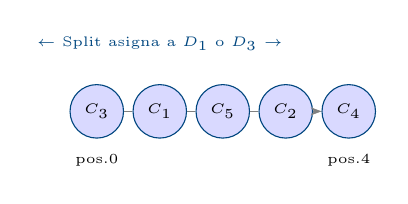
\begin{tikzpicture}[
        node/.style={circle, draw=myblue, fill=blue!15, minimum size=0.6cm, font=\tiny},
        dep/.style={circle, draw=myorange, fill=orange!20, minimum size=0.6cm, font=\tiny}
      ]
        \node[node] at (0,0) (c3) {$C_3$};
        \node[node] at (0.8,0) (c1) {$C_1$};
        \node[node] at (1.6,0) (c5) {$C_5$};
        \node[node] at (2.4,0) (c2) {$C_2$};
        \node[node] at (3.2,0) (c4) {$C_4$};
        \draw[-{Stealth},gray,very thin] (c3)--(c1)--(c5)--(c2)--(c4);
        \node[font=\tiny,below=0.08cm of c3] {pos.0};
        \node[font=\tiny,below=0.08cm of c4] {pos.4};
        \node[above=0.3cm of c1, font=\tiny, myblue] {$\leftarrow$ Split asigna a $D_1$ o $D_3$ $\rightarrow$};
      \end{tikzpicture}
      \end{center}
      \vspace{0.1em}
      \small El Split corta el CS en segmentos consecutivos y asigna cada segmento al depósito de menor costo.
    \end{column}
  \end{columns}
\end{frame}

\begin{frame}{MA$|$PM --- Algoritmo Split (Decodificación)}
  \begin{columns}[T,onlytextwidth]
    \begin{column}{0.52\textwidth}
      \begin{algorithm}[H]
        \caption{\small Split: CS $\to$ rutas óptimas}
        \begin{algorithmic}[1]\tiny
          \Require tour gigante CS$[0..n{-}1]$, depósitos abiertos $\mathcal{D}$, $Q$, dist.\ $d$, costo $F$
          \Ensure  costo de ruteo (sin apertura de depósitos)
          \State $dp[k] \gets +\infty\ \forall k$;\ $dp[0] \gets 0$
          \State $\textit{prev}[k] \gets -1$;\ $\textit{depot}[k] \gets$ nulo
          \For{$i \gets 0$ \textbf{to} $n{-}1$}
            \State cap $\gets 0$
            \For{$j \gets i$ \textbf{to} $n{-}1$}
              \State cap $\gets$ cap $+$ demanda$[$CS$[j]]$
              \If{cap $> Q$} \textbf{break} \EndIf
              \State mejor $\gets +\infty$;\ $d^* \gets$ nulo
              \ForAll{depósito $D \in \mathcal{D}$}
                \State $c \gets F + d[D][$CS$[i]] + \ldots + d[$CS$[j]][D]$
                \Comment{Held-Karp para CS[$i..j$] desde $D$}
                \If{$c <$ mejor} mejor $\gets c$;\ $d^* \gets D$ \EndIf
              \EndFor
              \If{$dp[i] + $ mejor $< dp[j+1]$}
                \State $dp[j{+}1] \gets dp[i]+$ mejor
                \State $\textit{prev}[j{+}1] \gets i$;\ $\textit{depot}[j{+}1] \gets d^*$
              \EndIf
            \EndFor
          \EndFor
          \State Reconstruir rutas retrocediendo con \textit{prev}[ ]
          \State \Return $\sum O(D_i \text{ abiertos}) + dp[n]$
        \end{algorithmic}
      \end{algorithm}
    \end{column}
    \begin{column}{0.46\textwidth}
      \textbf{Variables clave:}
      \vspace{0.2em}
      \begin{description}[\texttt{depot[k]}]\footnotesize
        \item[\texttt{dp[k]}] Costo mínimo de rutear los primeros $k$ clientes del tour CS
        \item[\texttt{i, j}] Inicio y fin del segmento actual (posiciones en CS)
        \item[\texttt{cap}] Demanda acumulada del segmento $[i..j]$
        \item[\texttt{prev[k]}] De dónde vino el mejor corte para llegar a $k$
        \item[\texttt{depot[k]}] Depósito óptimo para el segmento que termina en $k$
      \end{description}
      \vspace{0.3em}
      \begin{exampleblock}{Complejidad}\footnotesize
        $\mathcal{O}(n^2 \cdot m)$: para cada par $(i,j)$ se prueban $m$ depósitos. En la práctica muy rápido porque $Q$ limita el tamaño de los segmentos.
      \end{exampleblock}
    \end{column}
  \end{columns}
\end{frame}

\begin{frame}{MA$|$PM --- Búsqueda Local LS1}
  \begin{columns}[T,onlytextwidth]
    \begin{column}{0.50\textwidth}
      \begin{algorithm}[H]
        \caption{\small LS1: mejora por vecindades (\textit{first-improvement})}
        \begin{algorithmic}[1]\tiny
          \Require solución $s$ (rutas explícitas por depósito)
          \Ensure  $s$ mejorada localmente
          \State mejoró $\gets$ verdadero
          \While{mejoró}
            \State mejoró $\gets$ falso
            \For{operador $op \in \{$\textsc{move}, \textsc{swap}, \textsc{2-opt}$\}$}
              \ForAll{par de rutas $(r_1, r_2)$ (mismo o distinto depósito)}
                \State $\delta \gets$ ganancia de aplicar $op$ a $(r_1, r_2)$
                \If{$\delta < 0$} \Comment{mejora de costo}
                  \State aplicar $op$; recalcular costos
                  \State mejoró $\gets$ verdadero; \textbf{break}
                \EndIf
              \EndFor
              \If{mejoró} \textbf{break} \EndIf
            \EndFor
          \EndWhile
          \State \Return $s$
        \end{algorithmic}
      \end{algorithm}
    \end{column}
    \begin{column}{0.48\textwidth}
      \textbf{Tres vecindades aplicadas:}
      \vspace{0.3em}
      \begin{description}[\textsc{2-opt}]\footnotesize
        \item[\textsc{move}] Relocalizar un cliente: moverlo a otra posición en la misma ruta o a otra ruta (incluso de otro depósito)
        \item[\textsc{swap}] Intercambiar dos clientes de rutas del mismo o distinto depósito
        \item[\textsc{2-opt}] Inversión de subsecuencia intra-ruta; reconexión cruzada inter-ruta
      \end{description}
      \vspace{0.4em}
      \begin{block}{LS1 vs.\ LS2}\footnotesize
        \textbf{LS1}: aplica los 3 operadores sobre el cromosoma decodificado; actualiza el CS al terminar.\\
        \textbf{LS2}: igual pero aplica 2-opt también entre depósitos distintos (más costoso, menos frecuente).
      \end{block}
    \end{column}
  \end{columns}
\end{frame}

\begin{frame}{MA$|$PM --- OX Crossover y Gestión de Diversidad}
  \begin{columns}[T,onlytextwidth]
    \begin{column}{0.50\textwidth}
      \begin{algorithm}[H]
        \caption{\small OX Crossover + BPD}
        \begin{algorithmic}[1]\tiny
          \Require padres $P_1$, $P_2$ (cromosomas); umbral $\Delta$; población $\mathcal{P}$
          \Ensure  hijo $H$ o rechazo
          \State \textbf{Cruce DS}: seleccionar aleatoriamente de $P_1$ o $P_2$ por posición
          \State Elegir puntos de corte aleatorios $[a, b]$ en CS
          \State $H.CS[a..b] \gets P_1.CS[a..b]$
          \State Completar $H.CS$ con el orden de $P_2$, omitiendo duplicados
          \State Si DS inválido: \texttt{repair(H)}
          \State Evaluar $H$ con Split + LS1
          \ForAll{individuo $s \in \mathcal{P}$}
            \State $\text{BPD}(H, s) \gets |\text{pares}(H) \mathbin{\triangle} \text{pares}(s)|$
            \If{$\text{BPD}(H, s) < \Delta$}
              \State \Return rechazado \Comment{demasiado similar}
            \EndIf
          \EndFor
          \State Reemplazar el individuo de mayor costo en $\mathcal{P}$ con $H$
          \State \Return $H$
        \end{algorithmic}
      \end{algorithm}
    \end{column}
    \begin{column}{0.48\textwidth}
      \textbf{Broken Pairs Distance (BPD):}
      \[
        D(T,U) = |\,\text{pares}(T) \mathbin{\triangle} \text{pares}(U)\,|
      \]
      \footnotesize
      Donde \textit{pares}$(T)$ = conjunto de pares $(i,j)$ de clientes adyacentes en alguna ruta de $T$ (par simétrico: clave = $\{\min,\max\}$).
      \vspace{0.4em}
      \begin{block}{Ciclo de vida de la población}\footnotesize
        \begin{enumerate}
          \item Inicializar con NN y Clarke-Wright $+$ LS1
          \item Selección por torneo binario (fitness)
          \item Cruce OX $\to$ LS1 $\to$ BPD check
          \item Si \texttt{NbNoAdd} $>$ \texttt{MaxNbNoAdd}: bajar $\Delta$
          \item Si \texttt{NbAcc} $>$ \texttt{MaxNbAcc}: refrescar población
        \end{enumerate}
      \end{block}
    \end{column}
  \end{columns}
\end{frame}

% ============================================================
\section{Ejemplo Paso a Paso}

\begin{frame}{Ejemplo --- Instancia Mínima}
  \begin{columns}[T,onlytextwidth]
    \begin{column}{0.40\textwidth}
      \textbf{5 nodos sobre el eje $x$:}
      \vspace{0.4em}
      \begin{center}
      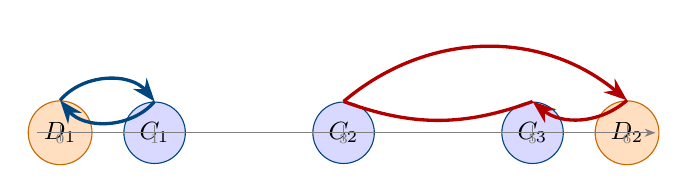
\begin{tikzpicture}[
        dep/.style={circle, draw=orange!80!black, fill=orange!25,
                    minimum size=0.65cm, font=\small\bfseries},
        cli/.style={circle, draw=myblue, fill=blue!15,
                    minimum size=0.65cm, font=\small}
      ]
        \def\sc{1.2}
        \node[dep] at (0*\sc,0) (D1) {$D_1$};
        \node[cli] at (1*\sc,0) (C1) {$C_1$};
        \node[cli] at (3*\sc,0) (C2) {$C_2$};
        \node[cli] at (5*\sc,0) (C3) {$C_3$};
        \node[dep] at (6*\sc,0) (D2) {$D_2$};
        \draw[gray, very thin, -{Stealth}] (-0.3,0)--(6.3*\sc,0);
        \foreach \x/\lab in {0/0,1/1,3/3,5/5,6/6}
          \draw[gray, very thin] (\x*\sc,-0.1)--(\x*\sc,0.1)
                node[below,font=\tiny,gray]{\lab};
        % Route 1: D1 - C1 - D1 (blue arc above)
        \draw[myblue, very thick, -{Stealth}]
              (D1.north) to[bend left=50] (C1.north);
        \draw[myblue, very thick, -{Stealth}]
              (C1.north) to[bend left=50] (D1.north);
        % Route 2: D2 - C2 - C3 - D2 (red arc above)
        \draw[red!70!black, very thick, -{Stealth}]
              (D2.north) to[bend left=40] (C3.north);
        \draw[red!70!black, very thick]
              (C3.north) to[bend left=20] (C2.north);
        \draw[red!70!black, very thick, -{Stealth}]
              (C2.north) to[bend left=40] (D2.north);
      \end{tikzpicture}
      \end{center}
      \vspace{0.3em}
      \footnotesize
      $Q=2$, $F=2$, $O=3$. Demanda de cada cliente $= 1$.\\[0.3em]
      \textbf{Ruta azul} $D_1\!\to\!C_1\!\to\!D_1$: $1+1+F=4$\\
      \textbf{Ruta roja} $D_2\!\to\!C_2\!\to\!C_3\!\to\!D_2$: $3+2+1+F=8$\\[0.3em]
      \textbf{Costo óptimo} $= O_1+O_2+4+8 = \mathbf{18}$
    \end{column}
    \begin{column}{0.58\textwidth}
      \textbf{Matriz de distancias:}
      \vspace{0.2em}
      \begin{center}\footnotesize
      \begin{tabular}{c|ccccc}
        \toprule
              & $D_1$ & $C_1$ & $C_2$ & $C_3$ & $D_2$ \\
        \midrule
        $D_1$ & 0 & 1 & 3 & 5 & 6 \\
        $C_1$ & 1 & 0 & 2 & 4 & 5 \\
        $C_2$ & 3 & 2 & 0 & 2 & 3 \\
        $C_3$ & 5 & 4 & 2 & 0 & 1 \\
        $D_2$ & 6 & 5 & 3 & 1 & 0 \\
        \bottomrule
      \end{tabular}
      \end{center}
      \vspace{0.4em}
      \textbf{Los tres algoritmos resuelven esta instancia:}
      \vspace{0.2em}
      \begin{center}\footnotesize
      \begin{tabular}{lccl}
        \toprule
        Algoritmo & Costo inicial & Costo final & Observación \\
        \midrule
        Fuerza Bruta & --- & \textbf{18} & Garantizado exacto \\
        ALNS         & 26  & \textbf{18} & 1\textsuperscript{a} iter.\ lo mejora \\
        MA$|$PM      & 19  & \textbf{18} & Split + OX lo encuentran \\
        \bottomrule
      \end{tabular}
      \end{center}
    \end{column}
  \end{columns}
\end{frame}

% ── Ejemplo: Fuerza Bruta ────────────────────────────────────
\begin{frame}{Ejemplo --- Fuerza Bruta paso a paso}
  \begin{columns}[T,onlytextwidth]
    \begin{column}{0.50\textwidth}
      \textbf{Caso A — Solo $D_1$ abierto:}
      \vspace{0.3em}
      \begin{center}\footnotesize
      \begin{tabular}{lll}
        \toprule
        Partición & Rutas desde $D_1$ & Costo total \\
        \midrule
        $\{C_1,C_2\}+\{C_3\}$ & $8+12$ & $O_1+20=\mathbf{23}$ \\
        $\{C_1\}+\{C_2,C_3\}$ & $4+12$ & $O_1+16=\mathbf{19}$ $\checkmark$ \\
        $\{C_1,C_3\}+\{C_2\}$ & $12+8$ & $O_1+20=\mathbf{23}$ \\
        \bottomrule
      \end{tabular}
      \end{center}
      \small Set-Cover DP elige $dp[111]=16$. \textbf{Mejor: 19.}

      \vspace{0.5em}
      \textbf{Caso B — Solo $D_2$ abierto:}
      \vspace{0.3em}
      \begin{center}\footnotesize
      \begin{tabular}{lll}
        \toprule
        Partición & Rutas desde $D_2$ & Costo total \\
        \midrule
        $\{C_1,C_2\}+\{C_3\}$ & $12+4$ & $O_2+16=\mathbf{19}$ $\checkmark$ \\
        $\{C_1\}+\{C_2,C_3\}$ & $12+8$ & $O_2+20=23$ \\
        \bottomrule
      \end{tabular}
      \end{center}
      \small \textbf{Mejor: 19.}
    \end{column}
    \begin{column}{0.48\textwidth}
      \textbf{Caso C — $D_1$ y $D_2$ abiertos:}
      \vspace{0.3em}
      \begin{center}\footnotesize
      \begin{tabular}{lrl}
        \toprule
        Asignación & Costo & \\
        \midrule
        $D_1{:}\{C_1\},\; D_2{:}\{C_2,C_3\}$ & $6+4+8=\mathbf{18}$ & $\checkmark$ \\
        $D_1{:}\{C_2\},\; D_2{:}\{C_1,C_3\}$ & $6+8+12=26$ & \\
        $D_1{:}\{C_3\},\; D_2{:}\{C_1,C_2\}$ & $6+12+12=30$ & \\
        $D_1{:}\{C_1,C_2\},\; D_2{:}\{C_3\}$ & $6+8+4=\mathbf{18}$ & $\checkmark$ \\
        $D_1{:}\{C_1,C_3\},\; D_2{:}\{C_2\}$ & $6+12+8=26$ & \\
        $D_1{:}\{C_2,C_3\},\; D_2{:}\{C_1\}$ & $6+12+12=30$ & \\
        \bottomrule
      \end{tabular}
      \end{center}
      \small \textbf{Mejor: 18.}

      \vspace{0.5em}
      \begin{alertblock}{Resultado exacto}\small
        $\min(19,\, 19,\, 18) = \mathbf{18}$\\
        Dos soluciones óptimas con ambos depósitos abiertos.
        La Fuerza Bruta \textbf{garantiza} que no existe mejor solución.
      \end{alertblock}
    \end{column}
  \end{columns}
\end{frame}

% ── Ejemplo: ALNS — Slide 1 ──────────────────────────────────
\begin{frame}{Ejemplo ALNS (1/3) --- Solución Inicial e Iteración 1}
  \begin{columns}[T,onlytextwidth]
    \begin{column}{0.50\textwidth}
      \begin{block}{Solución inicial $S_0$ (All-Open + greedy)}\footnotesize
        Todos los depósitos abiertos. Greedy asigna $C_3$ a $D_1$ (primer procesado).\\[0.2em]
        $D_1$: ruta $[C_1,C_3]$: $1{+}4{+}5{+}2 = 12$\quad
        $D_2$: ruta $[C_2]$: $3{+}3{+}2 = 8$\\[0.2em]
        $\text{Costo}(S_0) = O_1{+}O_2{+}12{+}8 = \mathbf{26}$
      \end{block}

      \vspace{0.2em}
      \textbf{Iter.\ 1 — \texttt{random\_removal}$(q{=}1)$:}
      \begin{itemize}\small
        \item Se extrae $C_3$ de la ruta $[C_1,C_3]$ de $D_1$
        \item Estado: $D_1{:}[C_1]$,\ $D_2{:}[C_2]$,\ \texttt{no\_asig}$=\{C_3\}$
      \end{itemize}

      \vspace{0.2em}
      \textbf{\texttt{greedy\_repair}: deltas para $C_3$}
      \vspace{0.1em}
      \begin{center}\footnotesize
      \begin{tabular}{lcc}
        \toprule
        Posición & Cálculo $\Delta$ & $\Delta$ \\
        \midrule
        Tras $C_1$ en $D_1$ &
          $4{+}5{-}1$ & $+8$ \\
        \textbf{Tras $C_2$ en $D_2$} &
          $2{+}1{-}3$ & $\mathbf{0}$ $\checkmark$ \\
        Nueva ruta $\{C_3\}$ en $D_2$ &
          $1{+}1{+}2$ & $+4$ \\
        \bottomrule
      \end{tabular}
      \end{center}
    \end{column}
    \begin{column}{0.48\textwidth}
      \textbf{Resultado: $C_3$ insertado tras $C_2$ en $D_2$ ($\Delta{=}0$):}
      \vspace{0.15em}
      \begin{center}\footnotesize
      \begin{tabular}{ll}
        \toprule
        Ruta & Costo \\
        \midrule
        $D_1\!\to\!C_1\!\to\!D_1{+}F$ & $1{+}1{+}2=4$ \\
        $D_2\!\to\!C_2\!\to\!C_3\!\to\!D_2{+}F$ & $3{+}2{+}1{+}2=8$ \\
        \midrule
        $\text{Costo}(S_1) = O_1{+}O_2{+}4{+}8$ & $\mathbf{18}$ \\
        \bottomrule
      \end{tabular}
      \end{center}

      \vspace{0.2em}
      \textbf{Criterio SA:}
      \[ \Delta E = 18 - 26 = -8 < 0 \;\Rightarrow\; \text{siempre aceptado} \]
      \footnotesize $S_1$ pasa a ser nuevo mejor $S^* = S_1$.
      Operadores \texttt{random\_removal} + \texttt{greedy\_repair} reciben $\sigma_1$.

      \vspace{0.15em}
      \begin{alertblock}{Resultado Iter.\ 1}\small
        Inserción con $\Delta{=}0$: $C_3$ ya estaba «de vuelta» por esa ruta, agregarlo a $D_2$ no incrementa recorrido.\\
        \textbf{De costo 26 a 18 en una sola iteración.}
      \end{alertblock}
    \end{column}
  \end{columns}
\end{frame}

% ── Ejemplo: ALNS — Slide 2 ──────────────────────────────────
\begin{frame}{Ejemplo ALNS (2/3) --- worst\_removal y regret2\_repair}
  \begin{columns}[T,onlytextwidth]
    \begin{column}{0.50\textwidth}
      \textbf{Iter.\ 2 — \texttt{worst\_removal} ($q{=}1$):}
      \vspace{0.2em}
      \begin{itemize}\small
        \item Estado $S_1$: $D_1{:}[C_1]$,\ $D_2{:}[C_2,C_3]$
        \item Se calcula el \textbf{ahorro} de extraer cada cliente:
      \end{itemize}
      \vspace{0.3em}
      \begin{center}\footnotesize
      \begin{tabular}{lcc}
        \toprule
        Cliente & Ruta actual & Ahorro (marginal) \\
        \midrule
        $C_1$ & $D_1{:}[C_1]$ solo & $4$ \\
        $C_2$ & $D_2{:}[C_2,C_3]$ & $4$ \\
        $C_3$ & $D_2{:}[C_2,C_3]$ & $0$ \\
        \bottomrule
      \end{tabular}
      \end{center}
      \vspace{0.2em}
      \footnotesize
      $C_2$: sin él, ruta queda $D_2{-}C_3{-}D_2$ (costo $4$). Ahorro $= 8{-}4{=}4$.\\[0.15em]
      $C_3$: sin él, ruta queda $D_2{-}C_2{-}D_2$ (costo $8$). Ahorro $= 8{-}8{=}0$.\\[0.3em]
      \small Empate $C_1{/}C_2$ (marginal $=4$); se elige $C_1$.
      \quad \texttt{no\_asig}$=\{C_1\}$.
    \end{column}
    \begin{column}{0.48\textwidth}
      \textbf{\texttt{regret2\_repair} para $C_1$:}
      \vspace{0.3em}
      \begin{center}\footnotesize
      \begin{tabular}{lcc}
        \toprule
        Opción de inserción & $\Delta$ costo & Rango \\
        \midrule
        Nueva ruta $D_1{:}[C_1]$ & $+4$ & $\Delta_1$ (mejor) \\
        Nueva ruta $D_2{:}[C_1]$ & $+12$ & $\Delta_2$ (segunda) \\
        \midrule
        Arrepentimiento & $12{-}4 = 8$ & alto \\
        \bottomrule
      \end{tabular}
      \end{center}
      \vspace{0.2em}
      \small $C_1$ vuelve a $D_1$.\quad $S_2 = S_1$, costo $\mathbf{18}$.

      \vspace{0.4em}
      \begin{block}{Greedy vs.\ Regret-2}\footnotesize
        \textbf{Greedy}: inserta el cliente de menor $\Delta$ inmediato (miope).\\[0.3em]
        \textbf{Regret-2}: prioriza el que \textit{más perdería} si espera tu turno. Con un solo no-asignado ambos coinciden.\\[0.3em]
        Ventaja de Regret-2: con \textbf{múltiples} no-asignados, inserta primero el de mayor diferencia $\Delta_2{-}\Delta_1$, evitando órdenes sub-óptimos.
      \end{block}
    \end{column}
  \end{columns}
\end{frame}

% ── Ejemplo: ALNS — Slide 3 ──────────────────────────────────
\begin{frame}{Ejemplo ALNS (3/3) --- depot\_closing y Limitación}
  \begin{columns}[T,onlytextwidth]
    \begin{column}{0.50\textwidth}
      \textbf{Iter.\ 3 — \texttt{depot\_closing}:}
      \vspace{0.2em}
      \begin{enumerate}\small
        \item Seleccionar depósito a cerrar $\to$ se elige $D_1$
        \item Ahorro por cierre:
              \[ -O_1 - \text{costo}[D_1{:}C_1] = -3 - 4 = -7 \]
        \item $C_1$ debe ir a $D_2$. Ruta $[C_2,C_3]$ llena ($Q{=}2$).\\[0.2em]
              Nueva ruta $D_2{:}[C_1]$:\\
              $d(D_2,C_1){+}d(C_1,D_2){+}F = 5{+}5{+}2 = 12$
        \item Costo incremental: $\Delta E = -7 + 12 = +5$
      \end{enumerate}
      \vspace{0.3em}
      \textbf{Decisión SA:}
      \[ P = e^{-\Delta E / T_3} = e^{-5/49800} \approx \mathbf{0.9999} \]
      \footnotesize $T_3 = 50000\cdot0.998^2 \approx 49800$.
      SA \textbf{acepta} (temperatura todavía alta).\\[0.2em]
      $S_3$: solo $D_2$ abierto, rutas $[C_2,C_3]{+}[C_1]$, costo $= \mathbf{23}$.
    \end{column}
    \begin{column}{0.48\textwidth}
      \begin{alertblock}{Limitación: cierre irreversible}\small
        Desde $S_3$, \textbf{$D_1$ está cerrado} y no puede reabrirse.\\[0.3em]
        Los reparadores (\texttt{greedy\_repair}, \texttt{regret2\_repair}) solo insertan clientes en \texttt{depositos\_abiertos}.\\[0.3em]
        Mínimo alcanzable desde $S_3$: costo $\mathbf{19}$.\\
        La solución óptima (costo $= 18$) requiere $D_1$ abierto.
      \end{alertblock}

      \vspace{0.4em}
      \begin{block}{¿Cómo el ALNS retorna 18?}\small
        \begin{itemize}
          \item La \textbf{mejor solución} $S^*{=}18$ se recuerda siempre
          \item Conforme $T \to 0$, SA rechaza retrocesos costosos
          \item ALNS retorna $S^*{=}18$ al finalizar las iteraciones
          \item Mejora futura: operador de \textit{reapertura} de depósitos
        \end{itemize}
      \end{block}
    \end{column}
  \end{columns}
\end{frame}

% ── Ejemplo: MA|PM — Slide 1 ─────────────────────────────────
\begin{frame}{Ejemplo MA$|$PM (1/5) --- Población Inicial y Split Chr1}
  \begin{columns}[T,onlytextwidth]
    \begin{column}{0.43\textwidth}
      \begin{block}{Población inicial}\footnotesize
        \begin{tabular}{lll}
          \toprule
          & DS & CS (giant tour) \\
          \midrule
          Chr1 & $[1,0]$ & $[C_2,C_3,C_1]$ \\
          Chr2 & $[0,1]$ & $[C_1,C_2,C_3]$ \\
          \bottomrule
        \end{tabular}\\[0.25em]
        DS$[i]{=}1$: dep.\ $i$ abierto. CS: tour gigante.
      \end{block}

      \vspace{0.2em}
      \textbf{DP del Split Chr1:}\\[0.05em]
      \footnotesize (DS$=[1,0]$, solo $D_1$, CS$=[C_2,C_3,C_1]$)
      \vspace{0.15em}
      \begin{center}\footnotesize
      \begin{tabular}{ccc}
        \toprule
        $dp[k]$ & Valor & Segmento ganador \\
        \midrule
        $dp[0]$ & $0$  & inicial \\
        $dp[1]$ & $8$  & $[0..0]\ \{C_2\}$ \\
        $dp[2]$ & $12$ & $[0..1]\ \{C_2,C_3\}$ \\
        $dp[3]$ & $\mathbf{16}$ & $[2..2]\ \{C_1\}$: $dp[2]{+}4$ \\
        \bottomrule
      \end{tabular}
      \end{center}
      \footnotesize \textit{Mejor:} $dp[3]{=}16 < dp[1]{+}12{=}20$.
    \end{column}
    \begin{column}{0.55\textwidth}
      \textbf{Costos por segmento desde $D_1$ ($F{=}2$):}
      \vspace{0.1em}
      \begin{center}\footnotesize
      \begin{tabular}{cll}
        \toprule
        Seg. & Clientes & $F+$recorrido \\
        \midrule
        $[0..0]$ & $\{C_2\}$     & $2{+}3{+}3=8$ \\
        $[0..1]$ & $\{C_2,C_3\}$ & $2{+}3{+}2{+}5=12$ \\
        $[1..1]$ & $\{C_3\}$     & $2{+}5{+}5=12$ \\
        $[1..2]$ & $\{C_3,C_1\}$ & $2{+}5{+}4{+}1=12$ \\
        $[2..2]$ & $\{C_1\}$     & $2{+}1{+}1=4$ \\
        \bottomrule
      \end{tabular}
      \end{center}

      \vspace{0.1em}
      \textbf{Rutas Chr1} (backtracking: $dp[3]{=}dp[2]{+}4$, $dp[2]{=}dp[0]{+}12$):
      \begin{itemize}\footnotesize
        \item Seg.\ $[2..2]{=}\{C_1\}$ en $D_1$: costo $4$
        \item Seg.\ $[0..1]{=}\{C_2,C_3\}$ en $D_1$: costo $12$
        \item Fitness Chr1 $= O_1 + dp[3] = 3+16 = \mathbf{19}$
      \end{itemize}

      \vspace{0.1em}
      \begin{block}{Idea del Split}\footnotesize
        El Split optimiza la \textbf{partición} del CS: para cada segmento prueba todos los depósitos disponibles y elige el de menor costo. Con solo $D_1$ activo, todas las rutas parten de $D_1$.
      \end{block}
    \end{column}
  \end{columns}
\end{frame}

% ── Ejemplo: MA|PM — Slide 2 ─────────────────────────────────
\begin{frame}{Ejemplo MA$|$PM (2/5) --- Split Chr2 y Búsqueda Local LS1}
  \begin{columns}[T,onlytextwidth]
    \begin{column}{0.50\textwidth}
      \textbf{Split Chr2:} DS$=[0,1]$ (solo $D_2$), CS$=[C_1,C_2,C_3]$:
      \vspace{0.15em}
      \begin{center}\footnotesize
      \begin{tabular}{cll}
        \toprule
        Seg. & Clientes & $F+$recorrido desde $D_2$ \\
        \midrule
        $[0..0]$ & $\{C_1\}$     & $2{+}5{+}5=12$ \\
        $[0..1]$ & $\{C_1,C_2\}$ & $2{+}5{+}2{+}3=12$ \\
        $[1..1]$ & $\{C_2\}$     & $2{+}3{+}3=8$ \\
        $[1..2]$ & $\{C_2,C_3\}$ & $2{+}3{+}2{+}1=8$ \\
        $[2..2]$ & $\{C_3\}$     & $2{+}1{+}1=4$ \\
        \bottomrule
      \end{tabular}
      \end{center}
      \vspace{0.1em}
      \begin{center}\footnotesize
      \begin{tabular}{ccc}
        \toprule
        $dp[k]$ & Valor & Segmento ganador \\
        \midrule
        $dp[0]$ & $0$  & inicial \\
        $dp[1]$ & $12$ & $[0..0]\ \{C_1\}$ \\
        $dp[2]$ & $12$ & $[0..1]\ \{C_1,C_2\}$ \\
        $dp[3]$ & $\mathbf{16}$ & $[2..2]\ \{C_3\}$: $dp[2]{+}4$ \\
        \bottomrule
      \end{tabular}
      \end{center}
      \small Rutas Chr2: $D_2{:}\{C_1,C_2\}{+}\{C_3\}$.\quad
      Fitness $= O_2{+}16 = \mathbf{19}$.
    \end{column}
    \begin{column}{0.48\textwidth}
      \textbf{Búsqueda Local LS1 sobre ambos cromosomas:}
      \vspace{0.15em}
      \begin{center}\footnotesize
      \begin{tabular}{llc}
        \toprule
        Cromo. & Movimiento & Costo \\
        \midrule
        Chr1 & Mover $C_2$: $\{C_3\}{+}\{C_1,C_2\}$ & $O_1{+}20=23$ \\
             & Mover $C_3$: $\{C_2\}{+}\{C_1,C_3\}$ & $O_1{+}20=23$ \\
             & Fusionar (dem.$=3>Q$) & infactible \\
        \midrule
        Chr2 & Mover $C_1$: $\{C_2\}{+}\{C_1,C_3\}$ & $O_2{+}20=23$ \\
             & Mover $C_2$: $\{C_1\}{+}\{C_2,C_3\}$ & $O_2{+}20=23$ \\
        \bottomrule
      \end{tabular}
      \end{center}
      \vspace{0.1em}
      \small \textbf{Ambos cromosomas son localmente óptimos: fitness $= 19$.}

      \vspace{0.2em}
      \begin{alertblock}{Mínimo local — necesitamos cruce}\small
        Ninguna vecindad LS1 puede mejorar individualmente. El \textbf{cruce OX} combinará el material genético de Chr1 (DS$=[1,0]$) y Chr2 (DS$=[0,1]$) para generar un hijo con nuevas combinaciones y escapar del mínimo local de $19$.
      \end{alertblock}
    \end{column}
  \end{columns}
\end{frame}

% ── Ejemplo: MA|PM — Slide 3 ─────────────────────────────────
% ── Ejemplo: MA|PM — Slide 3 ─────────────────────────────────
\begin{frame}{Ejemplo MA$|$PM (3/5) --- OX Crossover y Resultado}
  \begin{columns}[T,onlytextwidth]
    \begin{column}{0.48\textwidth}
      \textbf{OX Crossover} ($P_1{=}$Chr1, $P_2{=}$Chr2, corte $[0..0]$):
      \vspace{0.3em}
      \begin{enumerate}\small
        \item Copiar $P_1[0..0]{=}[C_2]$ al hijo en pos.\ 0
        \item Recorrer $P_2{=}[C_1,\mathbf{C_2},C_3]$, omitir $\{C_2\}$:\\
              queda $[C_1, C_3]$
        \item Hijo.CS $= [C_2,\; C_1,\; C_3]$
        \item Hijo.DS: DS$[0]$ de Chr1$=1$;\ DS$[1]$ de Chr2$=1$\\
              $\Rightarrow$ DS$=[1,1]$ (ambos depósitos abiertos)
      \end{enumerate}

      \vspace{0.5em}
      \begin{alertblock}{Clave del cruce}\small
        Ningún padre tenía DS$=[1,1]$:\\
        Chr1 tenía $[1,0]$ y Chr2 tenía $[0,1]$.\\[0.3em]
        El cruce \textbf{combinó ambos estados} y creó un hijo que puede usar los dos depósitos simultáneamente.
      \end{alertblock}
    \end{column}
    \begin{column}{0.50\textwidth}
      \textbf{Reconstrucción del hijo tras Split} ($dp[3]{=}12$):
      \vspace{0.2em}
      \begin{itemize}\small
        \item $dp[3]{=}12$: viene de $dp[2]{+}4$ → seg.\ $\{C_3\}$ asignado a $D_2$
        \item $dp[2]{=}8$: viene de $dp[0]{+}8$ → seg.\ $\{C_2,C_1\}$ asignado a $D_1$
      \end{itemize}
      \vspace{0.3em}
      \begin{center}\small
      \begin{tabular}{ll}
        \toprule
        Ruta & Costo \\
        \midrule
        $D_1\!\to\!C_2\!\to\!C_1\!\to\!D_1{+}F$ & $3{+}2{+}1{+}2=8$ \\
        $D_2\!\to\!C_3\!\to\!D_2{+}F$            & $1{+}1{+}2=4$ \\
        \midrule
        Fitness $= O_1{+}O_2{+}8{+}4$ & $= \mathbf{18}$ $\checkmark$ \\
        \bottomrule
      \end{tabular}
      \end{center}
      \vspace{0.3em}
      \begin{block}{¿Por qué bajó de 19 a 18?}\small
        El hijo heredó DS$=[1,1]$. El Split pudo asignar $\{C_3\}$ al depósito más cercano ($D_2$, distancia $1$) en vez del lejano $D_1$ (distancia $5$), reduciendo el costo total en $10$.
      \end{block}
    \end{column}
  \end{columns}
\end{frame}

% ── Ejemplo: MA|PM — Slide 4 ─────────────────────────────────
\begin{frame}{Ejemplo MA$|$PM (4/5) --- Split del Hijo (DP detallado)}

  % ── Comparación arriba, ancho completo ──
  \textbf{Comparación Chr1 / Chr2 / Hijo:}
  \vspace{0.1em}
  \begin{center}\footnotesize
  \begin{tabular}{lccc}
    \toprule
    & Chr1 & Chr2 & Hijo \\
    \midrule
    DS      & $[1,0]$         & $[0,1]$         & $[1,1]$ \\
    CS      & $[C_2,C_3,C_1]$ & $[C_1,C_2,C_3]$ & $[C_2,C_1,C_3]$ \\
    Fitness & $19$            & $19$            & $\mathbf{18}$ \\
    \bottomrule
  \end{tabular}
  \end{center}

  \vspace{0.2em}
  % ── DP table + bloque al mismo nivel ──
  \begin{columns}[T,onlytextwidth]
    \begin{column}{0.55\textwidth}
      \textbf{Split Hijo:} DS$=[1,1]$, CS$=[C_2,C_1,C_3]$ — se prueban \textbf{ambos} depósitos por segmento:
      \vspace{0.15em}
      \begin{center}\footnotesize
      \begin{tabular}{clcc}
        \toprule
        Seg. & Clientes & $D_1$ / $D_2$ (costo) & $dp$ \\
        \midrule
        $[0..0]$ & $\{C_2\}$     & $8$ / $8$ (empate)          & $dp[1]=8$ \\
        $[0..1]$ & $\{C_2,C_1\}$ & $\mathbf{8}$ / $12$         & $dp[2]=8$ \\
        $[1..1]$ & $\{C_1\}$     & $\mathbf{4}$ / $12$         & $\min(12,8)=8$ \\
        $[1..2]$ & $\{C_1,C_3\}$ & $12$ / $12$ (empate)        & $dp[3]=20$ \\
        $[2..2]$ & $\{C_3\}$     & $12$ / $\mathbf{4}$         & $\min(20,8{+}4)=\mathbf{12}$ \\
        \bottomrule
      \end{tabular}
      \end{center}
    \end{column}
    \begin{column}{0.43\textwidth}
      \begin{block}{Ventaja del DS$=[1,1]$}\footnotesize
        Chr1 y Chr2 solo usaban \textbf{un} depósito cada uno.\\[0.2em]
        El hijo evalúa \textbf{ambos}: el segmento $\{C_3\}$ cuesta $4$ desde $D_2$ vs.\ $12$ desde $D_1$.\\[0.2em]
        Costo total: $3{+}16=19 \;\to\; 3{+}3{+}12=\mathbf{18}$.
      \end{block}
    \end{column}
  \end{columns}
\end{frame}

% ── Ejemplo: MA|PM — Slide 4 ─────────────────────────────────
\begin{frame}{Ejemplo MA$|$PM (5/5) --- BPD y Convergencia al Óptimo}
  \begin{columns}[T,onlytextwidth]
    \begin{column}{0.50\textwidth}
      \textbf{Broken Pairs Distance (BPD):}
      \[
        D(T,U) = |\,\text{pares}(T) \mathbin{\triangle} \text{pares}(U)\,|
      \]
      \footnotesize
      \textit{pares}$(X)$ = pares de clientes adyacentes en rutas de $X$ (simétrico: $\{i,j\}$).
      \vspace{0.3em}
      \begin{center}\footnotesize
      \begin{tabular}{ll}
        \toprule
        Individuo & Pares adyacentes \\
        \midrule
        Chr1 & $\{(C_2,C_3)\}$ \\
        Chr2 & $\{(C_1,C_2)\}$ \\
        Hijo & $\{(C_2,C_1)\}=\{(C_1,C_2)\}$ \\
        \bottomrule
      \end{tabular}
      \end{center}
      \vspace{0.3em}
      \footnotesize
      $D(\text{hijo, Chr1}) = |\{(C_2,C_3)\}\triangle\{(C_1,C_2)\}| = 2 \ge \Delta{=}1$
      \quad $\checkmark$\\[0.3em]
      $D(\text{hijo, Chr2}) = |\{(C_1,C_2)\}\triangle\{(C_1,C_2)\}| = 0 < \Delta{=}1$
      \quad $\times$
    \end{column}
    \begin{column}{0.48\textwidth}
      \begin{alertblock}{Hijo rechazado por similitud}\small
        El hijo (fitness$=18$) es \textbf{rechazado}: comparte exactamente los mismos pares adyacentes que Chr2.\\[0.2em]
        $\texttt{NbNoAdd} \mathrel{+}= 1$
      \end{alertblock}

      \vspace{0.4em}
      \begin{block}{Mecanismo de recuperación}\small
        Cuando \texttt{NbNoAdd} supera \texttt{MaxNbNoAdd}, el umbral $\Delta$ baja a $0$.\\[0.3em]
        Con $\Delta{=}0$, el hijo se \textbf{acepta} y reemplaza al individuo de mayor costo (Chr1 o Chr2, ambos en $19$).\\[0.3em]
        \textbf{MA$|$PM converge al óptimo 18.}\\[0.2em]
        La gestión de diversidad BPD evita convergencia prematura, incluso cuando el mejor hijo encontrado es temporalmente rechazado.
      \end{block}
    \end{column}
  \end{columns}
\end{frame}

% ============================================================
\section{Validación contra Fuerza Bruta}

\begin{frame}{Validación --- Metodología}
  \begin{columns}[T,onlytextwidth]
    \begin{column}{0.52\textwidth}
      \textbf{¿Cómo validamos las metaheurísticas?}
      \vspace{0.3em}
      \begin{enumerate}\small
        \item Construimos instancias propias ($n=10\ldots20$, $m=2\text{ o }3$) con parámetros controlados
        \item Ejecutamos Fuerza Bruta exacta para obtener el \textbf{óptimo comprobado}
        \item Ejecutamos ALNS y MA$|$PM sobre las mismas instancias
        \item Comparamos: $\text{gap} = \dfrac{Z_{alg} - Z_{BF}}{Z_{BF}} \times 100\%$
      \end{enumerate}
      \vspace{0.4em}
      \begin{alertblock}{Criterio del evaluador}\small
        La Fuerza Bruta debe tardar al menos \textbf{30 minutos} para demostrar que el problema es computacionalmente intraterable y las metaheurísticas son necesarias.\\
        La instancia \texttt{coord20-2-1} tarda \textbf{28.9 minutos}.
      \end{alertblock}
    \end{column}
    \begin{column}{0.46\textwidth}
      \textbf{Escala de tiempos de la Fuerza Bruta:}
      \vspace{0.3em}
      \begin{center}\footnotesize
      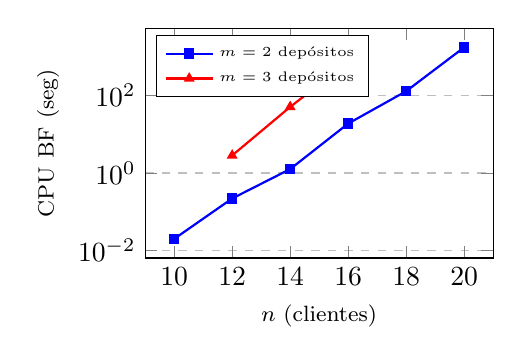
\begin{tikzpicture}
        \begin{axis}[
          width=6cm, height=4.5cm,
          xlabel={\footnotesize $n$ (clientes)},
          ylabel={\footnotesize CPU BF (seg)},
          xtick={10,12,14,16,18,20},
          ymode=log,
          ymajorgrids=true, grid style=dashed,
          legend pos=north west,
          legend style={font=\tiny},
          every axis plot/.append style={thick},
        ]
          \addplot[color=blue, mark=square*, mark size=1.5pt]
            coordinates {(10,0.02)(12,0.22)(14,1.26)(16,18.78)(18,128.40)(20,1733.0)};
          \addlegendentry{$m=2$ depósitos}
          \addplot[color=red, mark=triangle*, mark size=1.5pt]
            coordinates {(12,2.83)(14,50.46)(15,191.83)};
          \addlegendentry{$m=3$ depósitos}
        \end{axis}
      \end{tikzpicture}
      \end{center}
      \small Escala logarítmica. El tiempo crece \textbf{exponencialmente}
      con $n$ y $m$.
    \end{column}
  \end{columns}
\end{frame}

\begin{frame}{Validación --- Resultados vs.\ Óptimo Exacto}
  \begin{center}\footnotesize
  \begin{tabular}{lrr|rr|rr}
    \toprule
    Instancia & $n$ & $m$ &
    \multicolumn{2}{c|}{Fuerza Bruta} &
    \multicolumn{1}{c}{ALNS} &
    \multicolumn{1}{c}{MA$|$PM} \\
    \cmidrule(lr){4-5}
    & & & Óptimo & CPU (s) & Gap & Gap \\
    \midrule
    coord10-2-1 & 10 & 2 & 11\,576 & 0.02   & \textbf{0.00\%} & \textbf{0.00\%} \\
    coord10-2-2 & 10 & 2 & 15\,912 & 0.02   & \textbf{0.00\%} & \textbf{0.00\%} \\
    coord12-2-1 & 12 & 2 & 15\,123 & 0.22   & \textbf{0.00\%} & \textbf{0.00\%} \\
    coord14-2-1 & 14 & 2 & 17\,517 & 1.26   & \textbf{0.00\%} & \textbf{0.00\%} \\
    coord16-2-1 & 16 & 2 & 30\,324 & 18.78  & \textbf{0.00\%} & \textbf{0.00\%} \\
    coord18-2-1 & 18 & 2 & 31\,907 & 128.40 & \textbf{0.00\%} & \textbf{0.00\%} \\
    \rowcolor{yellow!25}
    coord20-2-1 & 20 & 2 & 35\,035 & \textbf{1733.0} (\textit{28.9 min}) & \textbf{0.00\%} & \textbf{0.00\%} \\
    \midrule
    coord12-3-1 & 12 & 3 & 17\,497 & 2.83   & \textcolor{red}{+5.86\%} & \textbf{0.00\%} \\
    coord14-3-1 & 14 & 3 & 20\,288 & 50.46  & \textcolor{red}{+5.82\%} & \textbf{0.00\%} \\
    coord15-3-1 & 15 & 3 & 21\,139 & 191.83 & \textbf{0.00\%} & \textbf{0.00\%} \\
    \midrule
    \textbf{Resumen} & & &
    \multicolumn{2}{l|}{BF exacto, pero exponencial} &
    Gap$\leq$5.9\% & Gap$=$0\% \\
    \bottomrule
  \end{tabular}
  \end{center}
  \vspace{0.2em}
  \begin{columns}[onlytextwidth]
    \begin{column}{0.60\textwidth}
      \small\textcolor{red}{\textbf{ALNS gap $>0$}} en instancias de 3 depósitos:
      el operador \texttt{depot\_closing} cierra un depósito que no debería,
      y los reparadores no pueden reabrirlo.
    \end{column}
    \begin{column}{0.38\textwidth}
      \small MA$|$PM: gap = 0\% en \textbf{todas} las instancias.
      Split siempre evalúa la combinación de depósitos abiertos óptima.
    \end{column}
  \end{columns}
\end{frame}

% ============================================================
\begin{frame}{Validador de Restricciones --- \tc{validar\_solucion()}}
  \begin{columns}[T,onlytextwidth]
    \begin{column}{0.46\textwidth}
      \textbf{¿Por qué existe?}\\[0.3em]
      \small La función objetivo $Z$ puede evaluarse sobre cualquier
      estado, incluso uno infactible (penalizaciones).
      El validador responde: \textit{¿cumple el modelo LRP exactamente?}

      \vspace{0.5em}
      \begin{block}{Restricciones verificadas}\footnotesize
        \begin{tabular}{@{}clp{3.1cm}@{}}
          \textbf{R1} & Ecs.\,2\&3 & Cada cliente visitado \textbf{exactamente una vez} \\
          \textbf{R2} & Ec.\,4     & Asignado a \textbf{un solo} depósito \\
          \textbf{R3} & Ec.\,5     & Rutas solo en \textbf{depósitos abiertos} \\
          \textbf{R4} & Ec.\,6     & Capacidad de \textbf{depósito} $\leq W_i$ \\
          \textbf{R5} & Ec.\,11    & Capacidad de \textbf{vehículo} $\leq Q$ \\
          \textbf{R6} & interna    & Coherencia \texttt{id\_deposito} \\
        \end{tabular}
      \end{block}
    \end{column}
    \begin{column}{0.52\textwidth}
      \textbf{Salida en consola (solución factible):}
      \vspace{0.2em}
      {\tiny\ttfamily
      \begin{tabular}{@{}l@{}}
      ========================================\\
      \phantom{xx}VALIDACIÓN DE RESTRICCIONES LRP\\
      ========================================\\
      n=10  m=2  |  Q=140  F=100\\
      Depósitos abiertos: 11 12 \ \ Rutas: 4\\
      ----------------------------------------\\
      R1: [OK]  10 clientes exactamente una vez\\
      R2: [OK]  Asignación uno-a-uno garantizada\\
      R3: [OK]  Todas las rutas en dep.\ abiertos\\
      R4: [OK]  Dep 11: 320.00 $\leq$ W=500\\
      R5: [OK]  Ruta 1: carga=130.00 $\leq$ Q=140\\
      ----------------------------------------\\
      Apertura:\ \ \ \ 4000.00\\
      Costo fijo:\ \ \ \ 400.00\\
      Costo viaje:\ 7176.00\\
      ========================================\\
      STATUS: SOLUCIÓN FACTIBLE  Z=11576.00\\
      ========================================\\
      \end{tabular}}

      \vspace{0.3em}
      \small\textbf{Tipo de retorno:} \tc{ResultadoValidacion}\\
      \footnotesize Contiene \tc{factible}, \tc{r1\_ok..r6\_ok},
      listas de violaciones y desglose de costos
      ($O_i$ + $F{\cdot}$rutas + viaje).
    \end{column}
  \end{columns}
\end{frame}

% ============================================================
\section{Resultados en Benchmark Prodhon}

\begin{frame}{Resultados en Benchmark Prodhon --- ALNS vs.\ MA$|$PM}
  \begin{columns}[T,onlytextwidth]
    \begin{column}{0.50\textwidth}
      \begin{center}\footnotesize
      \begin{tabular}{lrr}
        \toprule
        Grupo & Gap ALNS & Gap MA$|$PM \\
        \midrule
        $n=20$ (4 inst.)   & $-31.5\%$ & $-24.0\%$ \\
        $n=50$ (3 inst.)   & $-42.0\%$ & $-41.7\%$ \\
        $n=100$ (12 inst.) & $+8.3\%$  & $+59.0\%$ \\
        $n=200$ (6 inst.)  & $+29.5\%$ & $+129.9\%$\\
        \bottomrule
      \end{tabular}
      \end{center}
      \vspace{0.3em}
      \begin{center}
      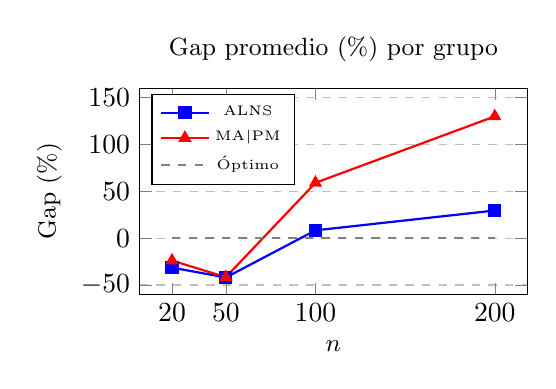
\begin{tikzpicture}
        \begin{axis}[
          width=6.5cm, height=4.2cm,
          title={\small Gap promedio (\%) por grupo},
          xlabel={\small $n$},
          ylabel={\small Gap (\%)},
          xtick={20,50,100,200},
          ymin=-60, ymax=160,
          legend pos=north west,
          legend style={font=\tiny},
          ymajorgrids=true, grid style=dashed,
          every axis plot/.append style={thick},
        ]
          \addplot[color=blue, mark=square*]
            coordinates {(20,-31.45)(50,-41.99)(100,8.30)(200,29.46)};
          \addplot[color=red, mark=triangle*]
            coordinates {(20,-23.95)(50,-41.67)(100,59.04)(200,129.92)};
          \addplot[color=gray, dashed, mark=none]
            coordinates {(20,0)(200,0)};
          \legend{ALNS, MA$|$PM, Óptimo}
        \end{axis}
      \end{tikzpicture}
      \end{center}
    \end{column}
    \begin{column}{0.48\textwidth}
      \textbf{Tiempos de CPU (promedio por grupo):}
      \vspace{0.2em}
      \begin{center}\footnotesize
      \begin{tabular}{lrr}
        \toprule
        Grupo & CPU ALNS & CPU MA$|$PM \\
        \midrule
        $n=20$  & $\sim$0.01\,s & $\sim$0.3\,s \\
        $n=50$  & $\sim$0.17\,s & $\sim$4\,s   \\
        $n=100$ & $\sim$0.6\,s  & $\sim$70\,s  \\
        $n=200$ & $\sim$7\,s    & $\sim$730\,s \\
        \bottomrule
      \end{tabular}
      \end{center}
      \vspace{0.3em}
      \begin{block}{Conclusión comparativa}\small
        \begin{itemize}
          \item $n \le 50$: equivalentes en calidad; ALNS 10$\times$ más rápido
          \item $n=100$: ALNS gana todas las instancias; $\sim$100$\times$ más rápido
          \item $n=200$: brecha drástica en ambas métricas
          \item Gap negativo = \textbf{mejor que el BKS registrado}
        \end{itemize}
      \end{block}
    \end{column}
  \end{columns}
\end{frame}

% ============================================================
\section{Conclusiones}

\begin{frame}{Conclusiones}
  \begin{columns}[T,onlytextwidth]
    \begin{column}{0.50\textwidth}
      \textbf{Lo que implementamos:}
      \begin{itemize}\small
        \item \textbf{Fuerza Bruta}: Held-Karp DP + Set-Cover DP, exacto para $n\le20$
        \item \textbf{ALNS}: 5 destructores + 2 reparadores, SA + ruleta adaptativa
        \item \textbf{MA$|$PM}: cromosoma DS+CS, Split $\mathcal{O}(n^2)$, NN/CW, OX, LS1/LS2
        \item Arquitectura modular C++17 con interfaz común \tc{IAlgoritmo}
      \end{itemize}
      \vspace{0.3em}
      \textbf{Validación rigurosa:}
      \begin{itemize}\small
        \item BF confirma el óptimo exacto hasta $n=20$, $m=3$
        \item BF en \texttt{coord20-2-1}: \textbf{28.9 min} $\Rightarrow$ justifica metaheurísticas
        \item MA$|$PM: gap = 0\% en todas las instancias validadas
        \item ALNS: gap $\le 5.9\%$ (limitación conocida por \texttt{depot\_closing})
      \end{itemize}
    \end{column}
    \begin{column}{0.48\textwidth}
      \textbf{Hallazgos experimentales (Prodhon):}
      \begin{itemize}\small
        \item $n \le 50$: ambos algoritmos superan el BKS registrado
        \item $n \ge 100$: ALNS domina en calidad y tiempo
        \item MA$|$PM escala mal: $\sim$100$\times$ más lento que ALNS en $n=100$
      \end{itemize}
      \vspace{0.4em}
      \begin{alertblock}{Trabajo futuro}
        \small Diseñar un algoritmo propio que combine la velocidad del ALNS con la robustez del MA$|$PM para la decisión de apertura de depósitos.
      \end{alertblock}
    \end{column}
  \end{columns}
\end{frame}

\end{document}
